
Serão descritas aqui algumas das tecnologias utilizadas na execução deste trabalho.

\section{Google BigQuery}

O \textit{Google BigQuery} é um produto disponível na plataforma de nuvem \textit{Google Cloud Platform} \cite{bigquery}, sendo uma tecnologia de armazém de dados gerenciada e altamente escalável. A interface de interação com os dados é a linguagem SQL. Se trata de um banco colunar capaz de lidar com dados da ordem de \textit{petabytes} de dados, e conta com ferramentas de segurança e criptografia nativas.

\begin{figure}[htb]
    \centering
    \caption{Interface do Google BigQuery para seleção de dados}
    \label{fig:bigquery}
    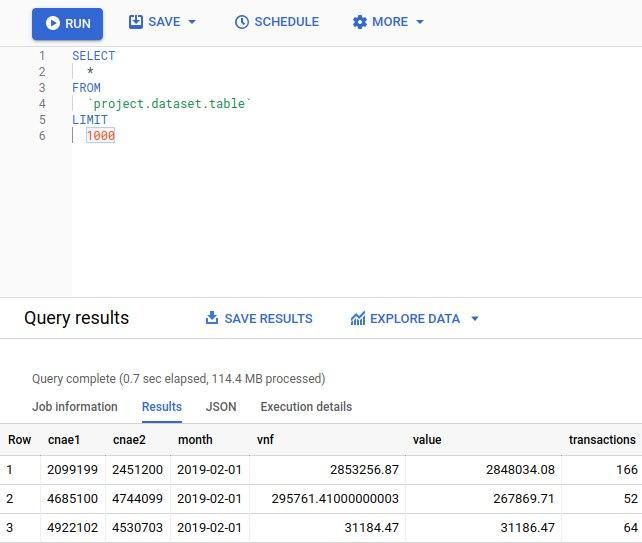
\includegraphics[scale=0.8]{images/bigquery.jpg}
    \fautor
\end{figure}

O \textit{Google BigQuery} é a tecnologia usada no armazenamento de dados do armazém de dados da empresa parceira.

\section{Google AI Platform Notebooks}

Outro produto disponível na \textit{Google Cloud Platform}, o \textit{Google AI Platform Notebooks} \cite{google-notebooks}, fornece um serviço gerenciado de integração segura com o ambiente JupyterLab, uma plataforma \textit{web} para aplicações usando Jupyter Notebook, uma aplicação \textit{web} para a criação e compartilhamento de códigos Python.

\section{Bibliotecas}

Neste trabalho foi utilizada a linguagem Python, com o auxílio das bibliotecas:

\begin{itemize}
    \item \textit{matplotlib} \cite{matplotlib}: para a visualização e criação de imagens.
    \item \textit{sklearn} \cite{sklearn}: para pré-processamento e execução de algoritmos de análise de dados e aprendizado de máquina.
    \item \textit{networkx} \cite{networkx}: para execução de algoritmos de processamento de redes.
    \item \textit{pandarallel} \cite{pandarallel}: para paralelização usando processamento \textit{multithread} para melhor escalabilidade.
\end{itemize}
